% 第7章：按照“人体估计—算法保护—机器人执行—任务验证”证据链组织。
% 建议使用 XeLaTeX 或 LuaLaTeX 编译。

\chapter{实验结果与分析}
\label{chap:experimental_results}

\section{实验数据与评价方法}
\label{sec:ch7_data_metrics}

本章围绕三个问题组织实验结果：第一，双接收器电磁系统能否准确、稳定地估计人体左臂
动作；第二，重定向、模型修正和安全保护是否按预期工作；第三，Unitree G1能否安全跟踪
目标并完成任务。开发期间用于定位故障的终端输出不逐条列入正文，只保留能够回答上述问题
的可复核证据。

系统开发和真机验证期间共保存135份可统一复核的
\texttt{g1\_arm\_tracking\_*.csv}，包含495420帧，记录时长合计
$9904.60\,\mathrm{s}$，约165.1 min。逐文件统计和SHA-256清单保存在项目实验记录目录中。
本章将数据分为表~\ref{tab:ch7_evidence_classes}所示的四类。

\begin{table}[htbp]
  \centering
  \caption{本章使用的证据类型}
  \label{tab:ch7_evidence_classes}
  \begin{tabularx}{\linewidth}{@{}lXX@{}}
    \toprule
    数据类型 & 用途 & 能否作为正式结论 \\
    \midrule
    正式协议重复 & R0、R1和R2各三次完整跟踪
      & 用于本章真机执行性能的主要定量结论 \\
    已审核预实验 & 有动作标签、终端记录和明确完成状态
      & 可报告定量结果，但注明为预实验 \\
    开发性全量记录 & 描述总体误差、覆盖时长和通信长尾
      & 不能据此计算正式成功率 \\
    功能性观察 & 说明算法分支、保护和异常是否真实出现
      & 可证明功能接入，不能替代配对统计 \\
    \bottomrule
  \end{tabularx}
\end{table}

真机跟踪误差定义为安全桥实际下发的命令角与编码器角之差：
\begin{equation}
  e_i(k)=q_{c,i}(k)-q_{a,i}(k),
  \label{eq:ch7_tracking_error}
\end{equation}
其中$q_{c,i}$为第$i$个关节经过限位和限速后的命令角，$q_{a,i}$为G1编码器角。据此
计算RMSE、P95绝对误差和最大绝对误差。该误差评价“机器人是否执行了安全命令”，不能
评价“人体动作是否估计正确”。人体估计精度必须使用独立视觉真值；50 Hz连续帧也不能
当作彼此独立的重复试次。

\section{电磁标定与重新佩戴稳定性}
\label{sec:ch7_calibration_repeatability}

\subsection{输入有效性检查}
\label{subsec:ch7_input_validity}

开发初期出现过大臂四元数模长约0.707、前臂保持1.000的异常。一次有效试验中，两接收器
四元数模长中位数均为1.000000，位置隐含运动范围为$73.3^\circ$，大臂和前臂报告的姿态
范围分别为$85.7^\circ$和$71.4^\circ$。异常试验中，大臂模长中位数降为0.711003，
大臂报告姿态范围只有$16.3^\circ$，而位置仍显示$71.7^\circ$运动；接收器对的平移和
方向残差上升至127.4 mm和$23.0^\circ$。

这说明该现象属于上游数据失效，而不是普通佩戴误差。采集节点随后加入0.95--1.05的模长
门控，异常数据整对丢弃，不通过强制归一化进入标定或真机。两次早期直臂刚性扫描虽然失败，
但后来确认测试中前臂发生了主动旋转，因此违反了刚性假设，不能据此判定接收器损坏。

\subsection{一次可用于真机的标定结果}
\label{subsec:ch7_calibration_snapshot}

一份用于后续受限真机测试的标定满足当时工程门槛，YAML中
\texttt{dry\_run\_only=false}。结果见表~\ref{tab:ch7_calibration_quality}。

\begin{table}[htbp]
  \centering
  \small
  \caption{一次可用于真机的安装标定结果}
  \label{tab:ch7_calibration_quality}
  \begin{tabularx}{\linewidth}{@{}Xrrl@{}}
    \toprule
    指标 & 实测值 & 工程门槛 & 判定 \\
    \midrule
    大臂静态位置RMS & 1.83 mm & $\leq3$ mm & 通过 \\
    前臂静态位置RMS & 2.68 mm & $\leq3$ mm & 通过 \\
    大臂静态姿态RMS & $0.57^\circ$ & $\leq3^\circ$ & 通过 \\
    前臂静态姿态RMS & $1.21^\circ$ & $\leq3^\circ$ & 通过 \\
    前臂旋转动作范围 & $75.92^\circ$ & $\geq55^\circ$ & 通过 \\
    前臂旋转轴拟合RMS & $2.17^\circ$ & $\leq15^\circ$ & 通过 \\
    前臂扭转重复最大误差 & $1.12^\circ$ & $\leq15^\circ$ & 通过 \\
    大臂参考方向最大误差 & $12.55^\circ$ & $\leq15^\circ$ & 通过但余量有限 \\
    前臂参考方向最大误差 & $13.35^\circ$ & $\leq15^\circ$ & 通过但接近上界 \\
    大臂位置模型RMS/最大误差 & 24.64/35.94 mm & $\leq35/65$ mm & 通过 \\
    \bottomrule
  \end{tabularx}
\end{table}

该次肘角修正增益为1.17697、偏置为$-0.99^\circ$；参考点修正后RMS为$2.98^\circ$，
最大绝对误差为$6.49^\circ$。结果证明至少有一次重新安装能够达到慢速真机验证要求，
但参考方向仍存在约$13^\circ$的模型--参考姿势残差。

\subsection{重新佩戴稳定性的证据边界}
\label{subsec:ch7_reinstallation_limit}

目前保存的多份标定NPZ包含被替代的尝试和不同测试分组，不能等同于多次“完全拆下--重新
佩戴--重新标定”的独立会话。因此现有结果只能证明标定流程能够产生可用参数，尚不能给出
跨安装合格率。正式结果仍需按统一协议完成至少5次独立重新佩戴，并以安装会话为统计单位
报告通过率和各残差的分布。

\section{人体姿态估计准确性}
\label{sec:ch7_human_accuracy}

\subsection{当前能够回答的问题}
\label{subsec:ch7_current_human_evidence}

现有标定残差、MuJoCo回放和真机日志能够说明输出连续、方向大体合理以及机器人可以执行
目标，但不能给出人体大臂方向、前臂方向和肘角的绝对误差。原因是人工参考姿势参与了参数
拟合，而真机CSV记录的是机器人命令与编码器响应，两者都不是独立人体真值。

因此，截至本章数据冻结时，人体姿态绝对精度尚不能被定量回答。本章不使用标定内部残差
冒充视觉误差，也不填写未经采集的结果。

\subsection{正式视觉真值实验应形成的结果}
\label{subsec:ch7_visual_ground_truth}

后续使用两台手机、刚性视觉标记和同步EM数据，对DOWN、直臂前举、直臂侧举、弯肘、
缓慢屈伸肘和弯肘转掌进行测量。视觉与EM分别计算大臂单位方向$\hat{\mathbf u}$、前臂
单位方向$\hat{\mathbf f}$和肘角$\theta_e$，误差定义为
\begin{align}
  e_u &= \arccos\!\left(\hat{\mathbf u}_{EM}^{T}\hat{\mathbf u}_{vis}\right), \\
  e_f &= \arccos\!\left(\hat{\mathbf f}_{EM}^{T}\hat{\mathbf f}_{vis}\right), \\
  e_e &= \theta_{e,EM}-\theta_{e,vis}.
  \label{eq:ch7_human_errors}
\end{align}

最终应报告三类误差的RMSE、中位数、P95和最大值，并给出至少一条视觉角与EM角的同步
时序曲线。这是证明“人体动作估计准不准”的核心实验，与G1关节跟踪实验相互独立。

\section{模型修正与碰撞保护}
\label{sec:ch7_model_collision}

\subsection{大臂位置模型与肘角修正}
\label{subsec:ch7_model_correction}

多轮测试表明，大臂仿射位置模型通常能够支持前举和侧举，但部分安装在前举过程中出现超过
50 mm的模型误差，并连续触发丢帧和停止发布。这一现象在人体距离机器人约2 m时仍出现，
说明原因更可能是安装变化、接收器局部运动、发射器相对位置或模型覆盖不足，不能简单归因于
机器人金属干扰。安全策略保持为：超出门槛时丢弃该帧，而不是为继续运动而放宽门槛。

肘角安装级仿射修正在标定参考点上把内部RMS降至$2.98^\circ$、最大误差降至
$6.49^\circ$，但参考点参与了参数拟合，因此仍需使用独立视觉动作比较修正前后误差，
才能证明泛化改善。

\subsection{躯干碰撞保护}
\label{subsec:ch7_torso_collision}

人体手臂贴近身体时，未保护的机器人目标可能使左臂进入躯干。加入25 mm躯干间隙过滤后，
MuJoCo胸前动作未再出现明显穿入，终端能够报告
\texttt{Torso collision protection activated}。过滤器只修改机器人安全目标，不反向
修改人体估计；找不到安全投影时保持上一安全目标。当前证据边界见
表~\ref{tab:ch7_model_collision_status}。

\begin{table}[htbp]
  \centering
  \small
  \caption{模型修正与碰撞保护的证据状态}
  \label{tab:ch7_model_collision_status}
  \begin{tabularx}{\linewidth}{@{}lXX@{}}
    \toprule
    模块 & 已有证据 & 尚缺少的正式结果 \\
    \midrule
    大臂仿射位置模型 & 有标定误差及在线门控记录
      & 同一视觉轨迹下与其他模型配对比较 \\
    肘角仿射修正 & 有标定内部修正前后结果
      & 独立动作的修正前后误差 \\
    碰撞过滤器 & MuJoCo功能通过，保护确实触发
      & 同轨迹C0/C1最小间隙和穿透帧数 \\
    \bottomrule
  \end{tabularx}
\end{table}

上述三项大部分可以使用已有NPZ离线回放完成，不需要重新占用G1。

\section{G1关节跟踪性能}
\label{sec:ch7_g1_tracking}

\subsection{网络、状态与平滑接管}
\label{subsec:ch7_takeover}

主机通过\texttt{enx6c1ff701509c}与G1的\texttt{192.168.123.161}通信，实测往返时间约
0.17--0.44 ms且无丢包。只读FSM监视器能够识别零力矩、阻尼、锁定站立和官方常规运控
状态。固定肘关节$5^\circ$试验中，肘角由$55.76^\circ$移动到约$60.50^\circ$，目标为
$60.76^\circ$，随后平滑返回并释放Arm SDK。

在所有关节目标固定为接管瞬间实测值时，Arm SDK权重分别升至0.10、0.20和0.25，三次
零动作接管诊断均通过，结果见表~\ref{tab:ch7_takeover_diagnostic}。

\begin{table}[htbp]
  \centering
  \caption{零动作Arm SDK接管诊断}
  \label{tab:ch7_takeover_diagnostic}
  \begin{tabular}{@{}rrrl@{}}
    \toprule
    最大权重 & 最大观测关节速度 & 最大关节漂移 & 结果 \\
    \midrule
    0.10 & 0.057 rad/s & $0.02^\circ$ & 通过，权重返回零 \\
    0.20 & 0.057 rad/s & $0.05^\circ$ & 通过，权重返回零 \\
    0.25 & 0.045 rad/s & $0.05^\circ$ & 通过，权重返回零 \\
    \bottomrule
  \end{tabular}
\end{table}

结果表明平滑接管本身不会造成明显关节跳变；权重达到1之后，接管渐变也不会继续增加正常
跟随延迟。

\subsection{单关节与小范围组合}
\label{subsec:ch7_single_small_multi}

单关节与小范围组合预实验共完成33轮，其中32轮完整结束，1轮因目标流陈旧中止。
完整试次共56750帧。单关节结果见表~\ref{tab:ch7_single_joint}。

\begin{table}[htbp]
  \centering
  \small
  \caption{G1左臂单关节慢速跟踪结果}
  \label{tab:ch7_single_joint}
  \begin{tabularx}{\linewidth}{@{}lXcrr@{}}
    \toprule
    关节 & 已覆盖范围 & 完整试次数 & RMSE范围 & 最大绝对误差 \\
    \midrule
    shoulder pitch & $5$--$20^\circ$单侧包络 & 5 & $0.88$--$1.35^\circ$ & $2.96^\circ$ \\
    shoulder roll & $5$--$20^\circ$包络 & 5 & $1.36$--$1.79^\circ$ & $3.39^\circ$ \\
    shoulder yaw & $\pm5$--$\pm15^\circ$ & 4 & $0.51$--$0.71^\circ$ & $1.26^\circ$ \\
    elbow & $5$--$45^\circ$，$3$--$5^\circ$/s & 6 & $0.27$--$0.60^\circ$ & $1.54^\circ$ \\
    wrist roll & $\pm5$--约$\pm30^\circ$ & 5 & $0.29$--$0.36^\circ$ & $0.90^\circ$ \\
    \bottomrule
  \end{tabularx}
\end{table}

肘、腕和肩yaw的RMSE均低于$0.8^\circ$，pitch最大RMSE为$1.35^\circ$。roll的RMSE
最高达到$1.79^\circ$，最大误差$3.39^\circ$，说明横向抬臂时负载影响最明显。所有完整
单关节试次均低于$5^\circ$硬停止阈值。

五关节$5^\circ$组合试验结果见表~\ref{tab:ch7_five_joint_small}。五关节同时达到至少
$2.5^\circ$幅值的累计时间为3.92 s，说明该记录包含真实协同动作，而非只有一个关节运动。

\begin{table}[htbp]
  \centering
  \caption{五关节$5^\circ$组合试验结果}
  \label{tab:ch7_five_joint_small}
  \begin{tabular}{@{}lrrrrr@{}}
    \toprule
    指标 & pitch & roll & yaw & elbow & wrist \\
    \midrule
    RMSE/$^\circ$ & 0.60 & 1.39 & 0.54 & 0.34 & 0.34 \\
    最大误差/$^\circ$ & 1.76 & 2.37 & 1.06 & 0.83 & 0.86 \\
    \bottomrule
  \end{tabular}
\end{table}

\subsection{逐级扩大范围}
\label{subsec:ch7_range_expansion}

扩大范围预实验保持最大命令速度$5^\circ$/s，逐级扩大五关节安全包络。第三档首次运行
因目标流陈旧中止，随后使用相同配置重试完成。结果见表~\ref{tab:ch7_range_expansion}。

\begin{table}[htbp]
  \centering
  \scriptsize
  \caption{五关节逐级扩大范围结果（RMSE/最大绝对误差）}
  \label{tab:ch7_range_expansion}
  \begin{tabularx}{\linewidth}{@{}Xrrrrrr@{}}
    \toprule
    P/R/Y/E/W包络 & pitch & roll & yaw & elbow & wrist & 最大倾角 \\
    \midrule
    20/20/15/30/20$^\circ$
      & 0.92/2.91 & 1.65/3.63 & 0.49/1.41 & 0.48/1.15 & 0.28/0.95 & $1.97^\circ$ \\
    25/20/15/35/25$^\circ$
      & 1.05/3.24 & 1.84/3.32 & 0.52/1.41 & 0.62/2.58 & 0.34/0.96 & $2.13^\circ$ \\
    30/25/15/45/30$^\circ$重试
      & 1.01/3.37 & 2.12/3.92 & 0.51/1.56 & 0.89/4.83 & 0.29/0.95 & $2.11^\circ$ \\
    \bottomrule
  \end{tabularx}
\end{table}

三档完整试验中所有关节最大误差均低于$5^\circ$。最大档elbow瞬时误差达到
$4.83^\circ$，接近硬停止阈值，但其RMSE为$0.89^\circ$、P95为$1.05^\circ$，说明峰值
属于短时动态滞后。最大档wrist相对幅值只达到$18.38^\circ$，不能据此声称已经验证完整
$30^\circ$范围。

\subsection{绝对对齐与正式R0/R1/R2}
\label{subsec:ch7_absolute_formal_trials}

后续系统从相对起点映射改为绝对对齐：接管后冻结人体目标，让机器人低速到达同一关节角，
误差进入容差后再开始跟随。该流程避免了接管瞬间的姿态跳变，但要求人体在对齐阶段保持
静止。pitch和roll还加入最大3 N$\cdot$m重力前馈；现有数据证明前馈可以安全启用，但没有
同一动作的严格开/关配对，因此不能声称已经量化其改善量。

正式试验按表~\ref{tab:ch7_formal_protocols}的协议进行。五关节包络
pitch/roll/yaw/elbow/wrist分别为$60/60/25/60/30^\circ$，pitch和roll重力前馈峰值均为
$3\,\mathrm{N\!\cdot\!m}$。每次佩戴后均执行相同标定流程；除协议规定的最大命令速度外，其余控制参数、
动作顺序和验收标准保持一致。表中帧数只包含绝对对齐完成后的正式跟踪段，不包含接管、对齐和
释放阶段。

\begin{table}[htbp]
  \centering
  \caption{正式R0/R1/R2真机试验协议}
  \label{tab:ch7_formal_protocols}
  \begin{tabularx}{\linewidth}{@{}lXrrrr@{}}
    \toprule
    协议 & 动作内容 & 跟踪时长 & 最大命令速度 & 重复数 & 有效帧数 \\
    \midrule
    R0 & 绝对对齐后保持当前五关节姿态 & 60 s & $5^\circ$/s & 3 & 9003 \\
    R1 & 固定顺序的五关节动态跟随 & 240 s & $5^\circ$/s & 3 & 36003 \\
    R2 & 与R1相同的五关节动态跟随 & 240 s & $8^\circ$/s & 3 & 36003 \\
    \bottomrule
  \end{tabularx}
\end{table}

九次有效试次共包含81009个正式跟踪帧，合计27 min。另有一次尝试在跟踪开始前因
人体肘部在绝对对齐期间移动$4.1^\circ$，超过$4.0^\circ$保持门槛而自动停止；该尝试没有进入
正式跟踪，因而不进入R0/R1/R2统计。

表~\ref{tab:ch7_formal_tracking}和表~\ref{tab:ch7_formal_p95}分别给出三次重复的RMSE和
P95绝对误差的均值及样本标准差。表~\ref{tab:ch7_formal_tracking}最后一列为该协议
所有关节和所有重复中的最大绝对误差。

\begin{table}[htbp]
  \centering
  \scriptsize
  \caption{正式R0/R1/R2跟踪RMSE（均值$\pm$样本标准差）}
  \label{tab:ch7_formal_tracking}
  \begin{tabular}{@{}lrrrrrr@{}}
    \toprule
    协议 & pitch & roll & yaw & elbow & wrist & 全局最大误差 \\
    \midrule
    R0 & $1.14\!\pm\!0.07$ & $0.76\!\pm\!0.09$ & $0.53\!\pm\!0.41$
       & $1.80\!\pm\!0.06$ & $0.17\!\pm\!0.05$ & $2.52^\circ$ \\
    R1 & $1.31\!\pm\!0.04$ & $1.06\!\pm\!0.04$ & $0.73\!\pm\!0.10$
       & $1.44\!\pm\!0.11$ & $0.31\!\pm\!0.03$ & $3.15^\circ$ \\
    R2 & $1.33\!\pm\!0.05$ & $1.08\!\pm\!0.01$ & $0.74\!\pm\!0.04$
       & $1.42\!\pm\!0.05$ & $0.35\!\pm\!0.03$ & $3.15^\circ$ \\
    \bottomrule
  \end{tabular}
\end{table}

\begin{table}[htbp]
  \centering
  \small
  \caption{正式R0/R1/R2跟踪P95绝对误差（均值$\pm$样本标准差）}
  \label{tab:ch7_formal_p95}
  \begin{tabular}{@{}lrrrrr@{}}
    \toprule
    协议 & pitch & roll & yaw & elbow & wrist \\
    \midrule
    R0 & $1.45\!\pm\!0.06$ & $0.87\!\pm\!0.17$ & $0.80\!\pm\!0.51$
       & $1.93\!\pm\!0.01$ & $0.30\!\pm\!0.05$ \\
    R1 & $2.20\!\pm\!0.10$ & $1.73\!\pm\!0.11$ & $1.44\!\pm\!0.35$
       & $1.96\!\pm\!0.06$ & $0.57\!\pm\!0.03$ \\
    R2 & $2.26\!\pm\!0.07$ & $2.01\!\pm\!0.15$ & $1.40\!\pm\!0.15$
       & $1.98\!\pm\!0.07$ & $0.65\!\pm\!0.02$ \\
    \bottomrule
  \end{tabular}
\end{table}

图~\ref{fig:ch7_formal_error_summary}将表~\ref{tab:ch7_formal_tracking}和
表~\ref{tab:ch7_formal_p95}中的结果可视化。柱高为三次独立重复的均值，误差棒为样本
标准差。静态R0的肘关节RMSE相对较大，而动态R1和R2的pitch与roll尾部误差相对较大；
但三种协议的全部均值仍低于$2.27^\circ$。

\begin{figure}[htbp]
  \centering
  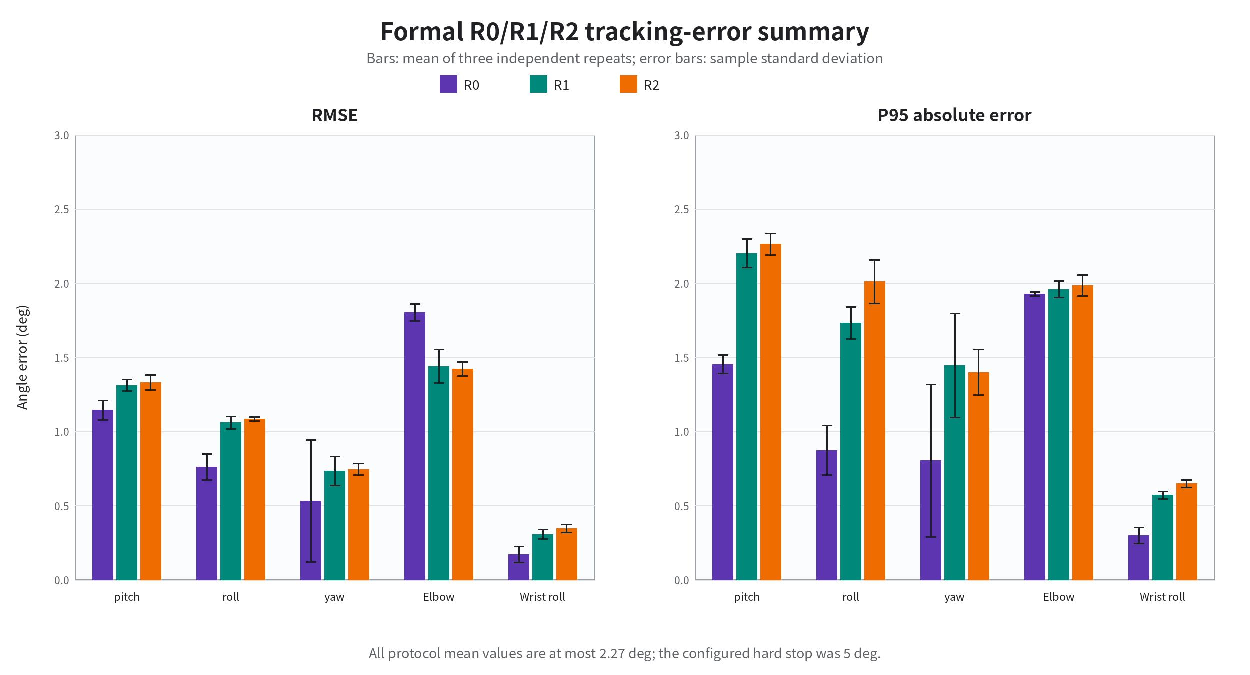
\includegraphics[width=\linewidth]{figures/g1_formal_error_summary.pdf}
  \caption{正式R0/R1/R2试验的五关节RMSE与P95绝对误差。误差棒为三次重复的样本标准差。}
  \label{fig:ch7_formal_error_summary}
\end{figure}

三种协议的所有关节RMSE均值均低于$1.81^\circ$，P95均值均低于$2.27^\circ$，最大绝对误差不超过
$3.16^\circ$，低于$5^\circ$硬停止门槛。R1与R2的各关节RMSE差异不超过$0.04^\circ$，
说明在本试验动作和安全包络内，将最大命令速度从$5^\circ$/s提高到$8^\circ$/s未导致明显的
跟踪误差增长。由于每组只有三次独立重复，该结论为描述性结论，不作显著性推断。

图~\ref{fig:ch7_formal_tracking_timeseries}给出R1和R2的安全命令角与编码器角时序。
为避免主观挑选，每个协议按五关节RMSE的算术平均值排序，选择居中的一次重复作为代表。
两种速度下五个关节的编码器曲线均紧邻安全命令曲线，较明显的偏差主要出现在动作换向和
快速过渡处，而不是持续发散。

\begin{figure}[htbp]
  \centering
  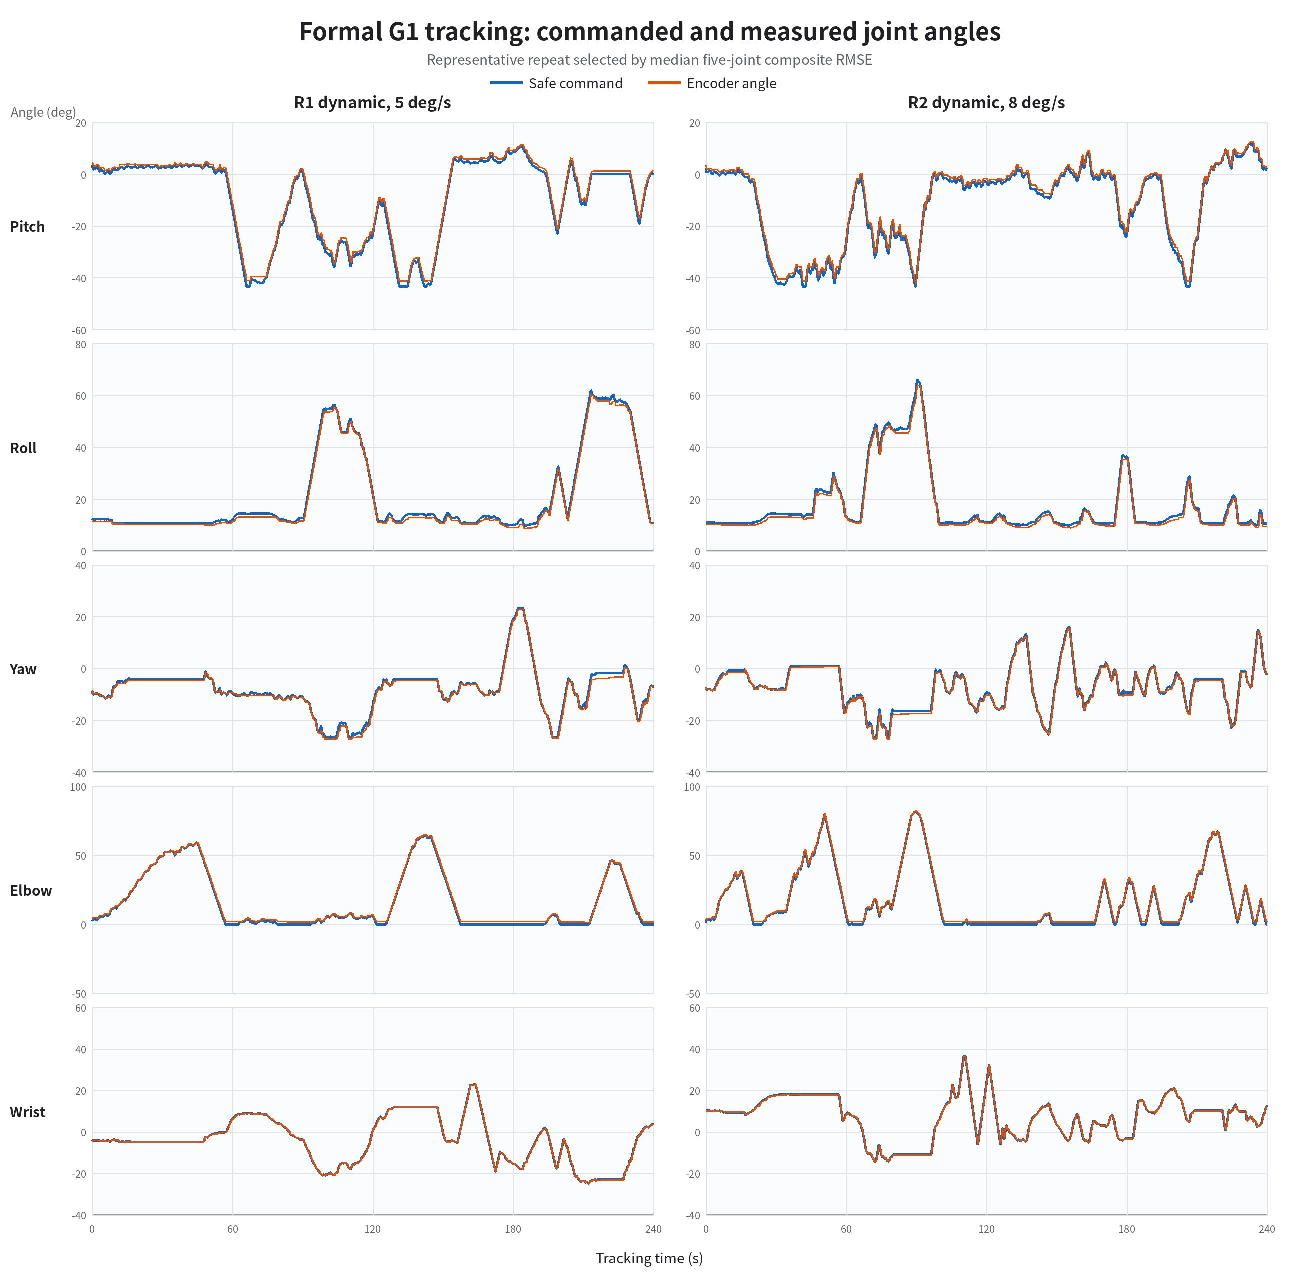
\includegraphics[width=\linewidth]{figures/g1_formal_tracking_timeseries.pdf}
  \caption{正式R1与R2代表性重复的安全命令角和编码器角。代表性重复由预先规定的
  五关节综合RMSE中位数规则自动选取。}
  \label{fig:ch7_formal_tracking_timeseries}
\end{figure}

安全裁剪按“人体源目标超出本轮允许包络”逐帧统计，结果见表~\ref{tab:ch7_formal_clipping}。
本研究采用“单次试验的任一单关节裁剪率小于5\%”作为小比例裁剪的工程验收条件。

\begin{table}[htbp]
  \centering
  \small
  \caption{正式试验单关节安全裁剪率（\%，均值$\pm$样本标准差）}
  \label{tab:ch7_formal_clipping}
  \begin{tabular}{@{}lrrrrrr@{}}
    \toprule
    协议 & pitch & roll & yaw & elbow & wrist & 单次最大值 \\
    \midrule
    R0 & $0.00\!\pm\!0.00$ & $0.00\!\pm\!0.00$ & $0.00\!\pm\!0.00$
       & $0.00\!\pm\!0.00$ & $0.00\!\pm\!0.00$ & 0.00 \\
    R1 & $1.37\!\pm\!2.22$ & $0.00\!\pm\!0.00$ & $2.45\!\pm\!1.87$
       & $0.00\!\pm\!0.00$ & $0.41\!\pm\!0.55$ & 4.61 \\
    R2 & $1.24\!\pm\!1.26$ & $0.31\!\pm\!0.54$ & $0.99\!\pm\!0.55$
       & $0.00\!\pm\!0.00$ & $0.74\!\pm\!0.80$ & 2.52 \\
    \bottomrule
  \end{tabular}
\end{table}

九次试验的任一单关节裁剪率都低于5\%，其中elbow在所有试次中均未裁剪。
裁剪不会使“安全命令--编码器”跟踪误差失效，但它表明机器人没有完整执行被裁掉的那一小段人体源目标，
因此表中同时报告跟踪误差和裁剪率，而不对原始数据进行事后修改。

正式跟踪段中，R0、R1和R2的UDP目标年龄P95分别为2.943、3.418和2.770 ms，
超过250 ms的帧比例分别为0.489\%、0.344\%和0.369\%；最大IMU倾角分别为
$1.96^\circ$、$2.57^\circ$和$2.58^\circ$。目标年龄的经验累积分布见
图~\ref{fig:ch7_formal_target_age_cdf}。这里的目标年龄是安全桥消费UDP目标时的数据年龄，
包含上游生成、传输和进程调度，不等同于网络往返时间。九次有效试次均完成正式跟踪、
平滑释放控制权并保存CSV。

\begin{figure}[htbp]
  \centering
  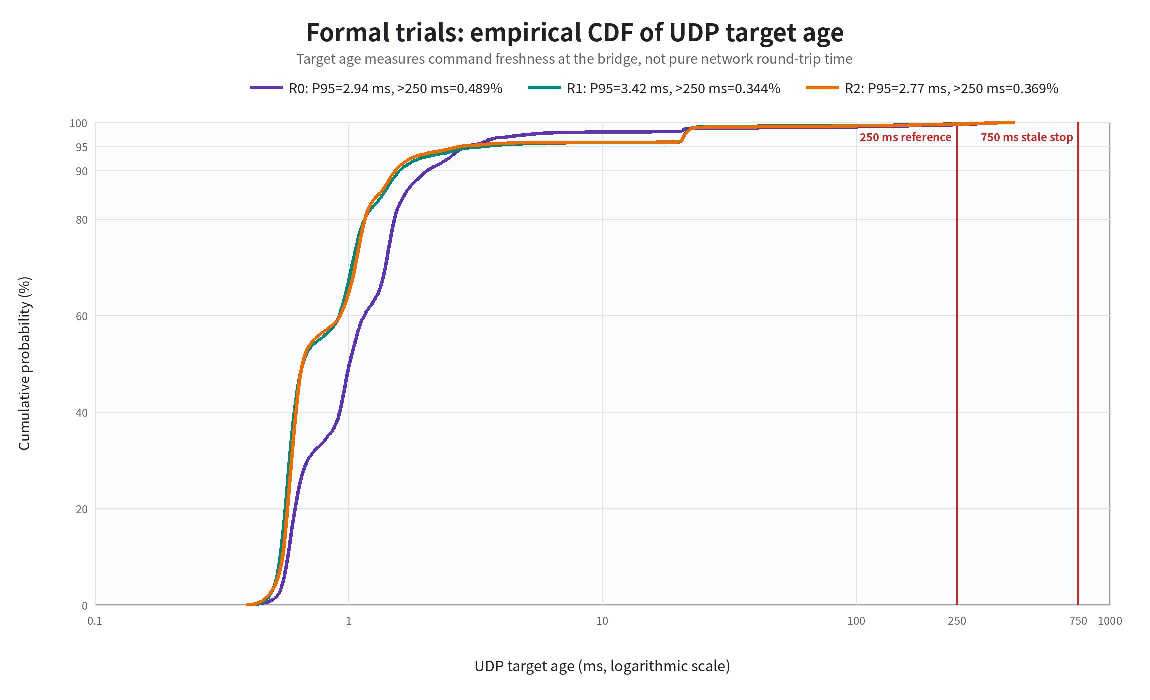
\includegraphics[width=\linewidth]{figures/g1_formal_target_age_cdf.pdf}
  \caption{正式R0/R1/R2跟踪段的UDP目标年龄经验累积分布。横轴采用对数尺度；竖线分别标出
  250 ms统计参考线和750 ms陈旧目标停止阈值。}
  \label{fig:ch7_formal_target_age_cdf}
\end{figure}

\subsection{实时性与安全停止}
\label{subsec:ch7_realtime_safety}

全部135份真机CSV的汇总见表~\ref{tab:ch7_all_logs}。该统计包含对齐阶段、开发中止和部分
关节试验，只描述执行链总体量级，不作为135次独立重复。

\begin{table}[htbp]
  \centering
  \caption{135份G1真机日志的全量统计}
  \label{tab:ch7_all_logs}
  \begin{tabularx}{0.82\linewidth}{@{}Xr@{}}
    \toprule
    指标 & 全量结果 \\
    \midrule
    文件/帧数/记录时长 & 135份/495420帧/165.1 min \\
    目标年龄中位数 & 0.802 ms \\
    目标年龄P95 & 4.278 ms \\
    目标年龄最大值 & 742.7 ms \\
    超过250 ms的帧 & 2637帧，0.532\% \\
    最大IMU倾角 & $2.96^\circ$ \\
    全量RMSE P/R/Y/E/W & $1.17/1.39/0.43/0.94/0.23^\circ$ \\
    全量最大误差 P/R/Y/E/W & $5.06/4.00/2.71/4.83/1.04^\circ$ \\
    \bottomrule
  \end{tabularx}
\end{table}

主体目标年龄处于毫秒量级，但存在0.38--0.74 s稀疏长尾。已确认的陈旧目标停止均执行了
“停止跟随--平滑降低Arm SDK权重--保存CSV”，随后相同或更大范围的重试可以完成。这证明
看门狗和释放流程实际介入；扩大超时只能减少停止次数，不能改善信息新鲜度。

\section{任务级验证}
\label{sec:ch7_task_validation}

截至本章数据冻结时，已完成的真机实验主要验证关节跟踪、安全包络和停止行为，尚未完成具有
明确环境目标和成功判据的正式任务级实验。因此，现有结果不能被写成“机器人已完成某项
应用任务”。

最终只需选择一个简单且可重复的任务，例如：机器人左手从初始区域移动至固定标靶区域，
保持2 s后返回。每次试验必须定义起点、目标区域、保持时间和失败条件，建议重复10次，并
报告成功率、完成时间、完成时间标准差、安全停止次数和失败原因。任务级演示与正式统计应
使用同一个任务，避免演示动作和论文任务成为两套无法对应的内容。

该实验需要G1、EM和电脑，但不要求同时使用双手机。手机系统用于评价人体姿态真值，任务级
实验用于评价整个系统是否能够完成可观察的目标，两者回答的问题不同。

\section{讨论}
\label{sec:ch7_discussion}

\subsection{人体估计误差与机器人执行误差必须分开}

当前最完整的数据是安全命令到G1编码器响应的执行误差。正式R0/R1/R2和多轮单关节实验能够
证明机器人跟踪链工作，但不能证明人体方向估计同样准确。只有完成双手机视觉对比后，才能
将“人体估计准确性”和“机器人执行准确性”连接成完整误差链。

\subsection{roll与大范围动作的负载影响}

单关节和扩大范围试验中，roll持续误差通常大于yaw、elbow和wrist；扩大包络后roll RMSE
进一步增加。该趋势与横向抬臂时重力矩增大一致，但现有前馈试验缺少同轨迹开/关配对，不能
把误差变化完全归因于重力，也不能量化3 N$\cdot$m前馈的净收益。

\subsection{安全裁剪不是数据错误}

正式R1和R2中的少量裁剪表示人体源目标短时超出了当次允许包络，安全桥主动限制机器人命令。
所有单次、单关节裁剪率都低于5\%，因此按本研究的工程验收条件保留为有效试次。裁剪后的机器人
跟踪误差仍然有效，但它评价的是安全命令而不是被裁掉的那部分人体源目标。因此论文同时报告命令跟踪误差和
裁剪比例，不修改原始数据消除裁剪。

\subsection{系统安全性证据}

四元数门控、位置模型门控、目标新鲜度看门狗、跟踪误差保护、机身状态检查、碰撞过滤以及
Arm SDK平滑释放均在实际测试中触发过。现有结果能够证明这些保护不是只存在于代码中，但
安全保护触发并不等于试验成功；正式结果必须分别报告完成试次和中止试次。

\section{局限性与剩余实验}
\label{sec:ch7_limitations_remaining}

目前第七章各结果模块的状态见表~\ref{tab:ch7_remaining_modules}。

\begin{table}[htbp]
  \centering
  \scriptsize
  \caption{第七章各结果模块的完成状态}
  \label{tab:ch7_remaining_modules}
  \begin{tabularx}{\linewidth}{@{}lXXX@{}}
    \toprule
    结果模块 & 所需设备 & 当前状态 & 最终需要补充 \\
    \midrule
    重新佩戴标定稳定性 & EM & 有多次开发经验，缺统一独立会话
      & 至少5次完整重装统计 \\
    人体姿态准确性 & 双手机+EM & 尚无独立视觉真值
      & 方向/肘角误差及同步曲线 \\
    模型与碰撞消融 & 电脑+已有NPZ & 功能已接入
      & 同轨迹离线对照 \\
    G1 R0/R1/R2 & G1+EM & 已完成；各三次正式重复
      & 不需要补测 \\
    任务级成功率 & G1+EM & 尚未正式完成
      & 一个任务约10次重复 \\
    \bottomrule
  \end{tabularx}
\end{table}

除此之外，当前研究仍局限于单名操作者、左臂、低至中等速度和实验室环境。直臂转掌不属于
本研究的评价动作，双手机系统自身也存在标定和遮挡误差。以上限制应在论文中明确陈述，而
不是通过增加缺少统一协议的开发日志来弱化。

\section{本章小结}
\label{sec:ch7_summary}

本章按照“人体估计--算法保护--机器人执行--任务验证”的证据链重新整理已有实验。电磁输入
门控能够识别四元数模长约0.707的异常；至少一次安装标定满足慢速真机要求，但跨安装稳定性
和人体绝对精度仍需正式重复佩戴与双手机实验确认。大臂位置模型门控和25 mm躯干碰撞保护
均已在开发试验中观察到实际作用。

G1侧已经完成平滑接管、单关节、多关节、逐级扩大范围和绝对对齐，
并完成R0、R1和R2各三次正式重复。正式数据共包含81009帧、27 min，所有关节RMSE
低于$1.81^\circ$，P95低于$2.27^\circ$，全局最大误差不超过$3.16^\circ$。R1和R2的跟踪误差
接近，表明在本试验范围内将最大命令速度从$5^\circ$/s提高到$8^\circ$/s未造成明显性能下降。
全部135份日志共覆盖约165.1 min，目标年龄中位数为0.802 ms，看门狗能够在目标陈旧时停止跟随并平滑释放控制。

因此，现有证据较强地支持G1执行链和安全链的可行性，但尚不能完成对人体绝对精度和任务
成功率的最终回答。后续工作的优先级应为：双手机人体真值和一个固定任务的10次验证；
其余模型与碰撞对照可使用现有数据离线完成。
